\documentclass{bioinfo}
\copyrightyear{2005}
\pubyear{2005}

\begin{document}
\firstpage{1}

\title[Application Note]{bioWeb3D: an online webGL 3D data visualisation tool}
\author[Pettit \textit{et~al}]{Jean-Baptiste Pettit\,$^{*}$ and John C. Marioni\footnote{to whom correspondence should be addressed}}
\address{EMBL-EBI, European Molecular Biology Laboratory - European Bioinformatics Institute, Cambridge, CB10 1SD, UK}

\history{Received on XXXXX; revised on XXXXX; accepted on XXXXX}

\editor{Associate Editor: XXXXXXX}

\maketitle

\begin{abstract}

\section{Summary:}
An online HTML5/webGL based 3D visualisation tool has been developed to allow biologists to quickly and easily view interactive and customizable three dimensional representations of their data along with multiple layers of information. Using the WebGL library Three.js written in Javascript, bioWeb3D allows the simultaneous visualisation of multiple large datasets inputted via a simple JSON file, which can be read and analysed locally thanks to HTML5 capabilities.

\section{Availability:}
http://www.ebi.ac.uk/$\sim$jbpettit/bioWeb3D \\ https://github.com/jibooo/bioWeb3D

\section{Contact:} \href{jbpettit@ebi.ac.uk}{jbpettit@ebi.ac.uk}, \href{marioni@ebi.ac.uk}{marioni@ebi.ac.uk}
\end{abstract}

\section{Introduction}

Visualisation is a key feature in the analysis of large biological datasets, especially when analysing organized structures with distinct sub-clusters \citep{Rubel10}. This is particularly important when analysing 3-Dimensional (3D) datasets, which is becoming more and more common. While various visualisation tools have been developed, they have typically been available via a locally installed piece of software such as BioLayout Express$^{3D}$\citep{Freeman07}, Arena3D \citep{Pavlopoulos08},  3D Genome Tuner \citep{Wang09}, the Allen Brain Atlas \citep{Lein07} or Cytoscape \citep{Shannon03}. Other 3D visualisation tools have been built online and are accessible through the browser directly, such as AstexViewer \citep{Hartshorn02}, which is utilised by the Protein Databank Europe via a Java Applet. More recently, visualisation tools developed using HTML5/WebGL capabilities have been described, although they have focused on very specific applications, such as analysing radiology data  \citep{Dinesh12}. However, no tool has allowed biologists to view their own 3D data directly online in an easy, fast, secure and interactive way. Using webGL and the JavaScript 3D library Three.js, bioWeb3D aims to be a simple, generic, tool for visualising such data.



\section{Technological overview}

bioWeb3D allows the representation of any 3D dataset by defining only two file formats, which enables the user to quickly upload their own datasets to their browser. The format of these files is based on JSON, a widely used structured format on the web \citep{Wilde07}.\\
The first file type contains the coordinates of every point in the dataset, while the second describes one or several information layers that can be associated with the points defined in the first file. For example, if each point defines the location of a cell within a tissue, the second file could describe whether a particular gene is expressed in each cell. \\
Datasets can be viewed and compared in up to four ``worlds" (each world refers to a separate visualisation sub-window) at the same time. Although web based, the application, fully written in Javascript, does not need to send any data to the host server. Instead the modern internet browser's local file system reading capabilities are used through the HTML 5 FileReader functionality. This allows the application to handle, in a very short period of time, large datasets while ensuring that the privacy of the data is maintained.\\
Although the focus is on making bioWeb3D simple and easy to use, some options are available to customise how datasets are represented. For example, the application can be used to visualise sequential information, such as 3D protein structures, in which case links can be drawn between the points. In other cases, such as when a population of cells are considered, the points can be left unlinked as individual particles. The information layers are visualised by colouring the 3D points according to the class that each point belongs to.
\subsection{Defining the input file format}
The JSON format has been chosen because of its rigorous structure, which allows fast Javascript object generation within the browser interpreter. Compared to other data-interchange languages, such as XML, JSON is also easily human readable thanks to a light-weight syntax. It is also supported by all of the primary internet browsers.\\
The {\it{dataset}} file should have a root object called ``dataset" which contains: 
\begin{itemize}
\item{The ``name" property of the dataset (\textit{e.g.}, ``my dataset").}
\item{The ``chain" parameter which has to be set to \textit{true} if the points should be linked, to \textit{false} otherwise (optional) the default value is \textit{false}). The data will be considered sequential, each point linked to the next in the dataset.}
\item{The ``points" property, which is a two dimensional array representing a list of (x,y,z) vectors that define the co-ordinates of the points.}
\end{itemize}

The {\it{information layer}} files must have a root element named  ``information". Since one information file can define multiple information sets, the structure below ``information" is a list. Each element of the list is structured as follows :
\begin{itemize}
\item{ The ``name" property (optional).}
\item{The ``numClass" property, which indicates the number of different classes the data will be assigned to.}
\item{The ``labels" property, which defines a list of names for the ``numClass" classes previously defined (optional).}
\item{The ``values" property, which defines the class of each point in the dataset. As points do not have single IDs, this property must be in the same order and have the same length as the points defined in the {\it{dataset}} file.}
\end{itemize}
Exact specifications and examples of the file formats can be found on the bioWeb3D gitHub repository wiki and in the supplementary materials. Since many biological results are in fact stored as CSV files we also provide easy to use Perl scripts that can quickly generate JSON files from CSV data. These scripts are also available from the GitHub repository.


\begin{figure}[h!]%figure1
\centerline{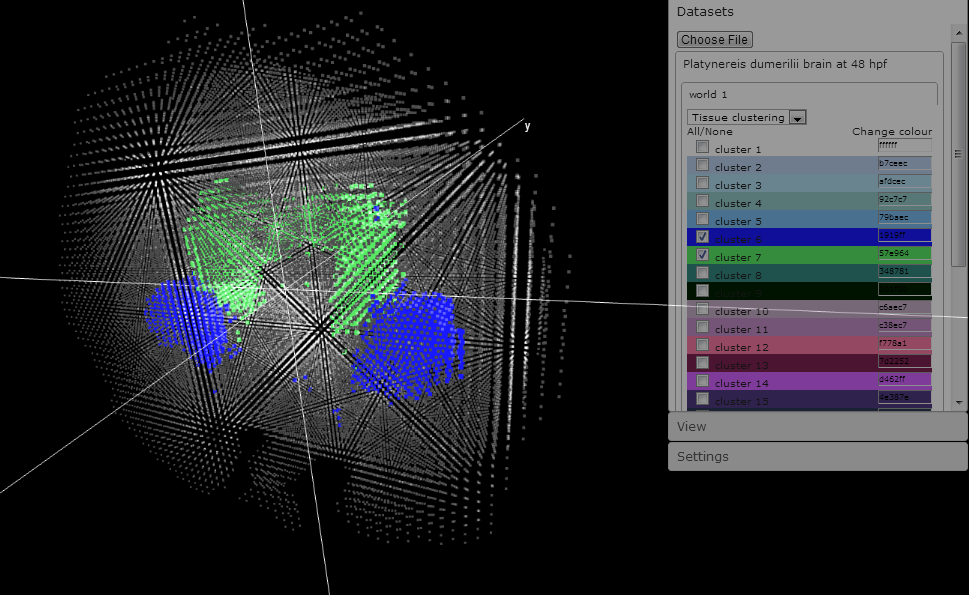
\includegraphics[totalheight=0.2\textheight]{fig1.png}}
\caption{An example of the application of bioWeb3D. The 3D location of cells within the brain of the marine annelid {\it{Platynereis dumerilii}} is shown. Two classes are displayed (in green and blue) along with the shadow of the remaining cells.The User interface is visible on the right of the screen and can be hidden with a ``show/hide" button located on the bottom left. Data for this figure was taken from \citep{Tomer10}.}\label{fig:01}
\end{figure}

\subsection{User interface}
The user can interact with the visualisation via an interface on the right of the screen (Figure 1), which contains three panels. In the ``dataset" panel, the user can choose the {\it{datasets}} and {\it{information layer}} files that should be represented in each world. This panel also allows the user to show/hide specific classes of the selected information layers. Each dataset file entered will create a new sub-panel where the user can input {\it{information layer}} files for each world. Selecting an {\it{information layer}} in the drop-down list will display the data in the current world and generate a list of classes that the user can modify regarding their visibility and colour. The ``View" panel enables the user to choose which of the worlds are shown on the screen, ranging from 1 to 4 simultaneous worlds (Supplementary Fig 1). Finally, the ``Settings" panel provides the user with a number of options that affect all the worlds and all datasets, such as allowing the axes scales to be modified.


\section{Discussion}
	\subsection{bioWeb3D and local software}
Many 3D visualisation software tools, most of which require local installation, exist and provide similar functionalities with standard 3D format input such as Wavefront .OBJ. Some are extremely generic and powerful but can have a steep learning curve like Blender. However, these tools are not typically oriented towards a scientific audience. Moreover, those that are more focused on science are often targeted towards a very specific application, especially in medical sciences \citep{Wang09}. In this context we believe that bioWeb3D can be useful as it is completely generic and web based. It should also be noted that recent browser improvements regarding GPU acceleration through the webGL paradigm allow bioWeb3D to visualise several hundred thousand three dimensional data points and to interact with then with perfect fluidity even on a laptop. In that regard browsers are competing directly with local software. Additionally, local software is usually platform specific, which is not the case for web based applications.

	\subsection{bioWeb3D and Java Applets}
As mentioned previously, web based 3D visualisation tools currently exist mainly in the form of Java Applets. This technology has attracted much criticism in 2012 regarding security flaws, leading the ``United States Computer Emergency Readiness Team" to advise that all Java Applets should be disabled due to current and future Java vulnerabilities (http://www.kb.cert.org/vuls/id/636312). The development of WebGL technology is viewed by many as a candidate for replacing Applets. 

	\subsection{Current limitations}
The main current limitation of a webGL based application is the machine and browser compatibility. Only computers with fairly recent graphic cards will be able to run a 3D environment. It should also be noted that Microsoft has notified the developer community that Internet Explorer is not scheduled to support WebGL in the near future. However, importantly, Chrome, Firefox, Safari and Opera all now support webGL applications (http://caniuse.com/webgl).



\section*{Acknowledgement}
The authors would like to acknowledge Samuel Croset, Tom Oldfield, Konrad Rudolph and Sergio Martinez Cuesta for helpful discussion and criticism as well as Ricardo Cabello the creator of the JavaScript library Three.js.

%\bibliographystyle{natbib}
%\bibliographystyle{achemnat}
%\bibliographystyle{plainnat}
%\bibliographystyle{abbrv}
%\bibliographystyle{bioinformatics}

%\bibliographystyle{plain}

%\bibliography{Document}

\begin{thebibliography}{}

\bibitem[Freeman {\it et~al}., 2007]{Freeman07} Freeman T.C., Goldovsky L., Brosch M., van Dongen S., Mazière P., Grocock R.J., Freilich S., Thornton J., Enright A.J. (2007). Construction, visualisation, and clustering of transcription networks from microarray expression data. {\it{PLoS Comput Biol.}}, {\bf{3(10)}}:2032-42.

\bibitem[Hartshorn, 2002]{Hartshorn02} Hartshorn M.J. (2002). AstexViewer: a visualisation aid for structure-based drug design. {\it{Journal of Computer-aided Molecule Design}} {\bf{16}}:871-881.

\bibitem[Kulkarni {\it et~al}., 2012]{Dinesh12} Kulkarni D.B., Doijade M.M., Devrukhkar C.S., Zilpe G.R. and Surana R.R. (2012). NetraRIS - a Web based DICOM Viewer. {\it{International Journal of Computer Applications}}.{\bf{48}}:40-44.

\bibitem[Lein {\it et~al}., 2007]{Lein07} Lein E.S., Hawrylycz M.J., Ao N., Ayres M., Bensinger A., Bernard A., Boe A.F., Boguski M.S., Brockway K.S., Byrnes E.J., {\it{et al.}}. (2007). Genome-wide atlas of gene expression in the adult mouse brain., {\it Nature}, {\bf{445}}:168-176.

\bibitem[Pavlopoulos {\it et~al}., 2008]{Pavlopoulos08} Pavlopoulos G.A., O'Donoghue S.I., Satagopam V.P., Soldatos T.G., Pafilis E. and Schneider R. (2008). Arena3D: visualisation of biological networks in 3D., {\it BMC Systems Biology}, {\bf{2}}:104.

\bibitem[Rubel {\it et~al}., 2010]{Rubel10} Rubel O., Weber G.H., Huang M.Y., Bethel E.W., Biggin M.D., Fowlkes C.C., Luengo Hendriks C.L., Ker\"{a}nen S.V., Eisen M.B., Knowles D.W., {\it{et al.}} (2010). Integrating Data Clustering and visualisation for the Analysis of 3D Gene Expression Data. {\it IEEE/ACM Trans Comput Biol Bioinform}, {\bf{7}}:64-79.

\bibitem[Tomer {\it et~al}., 2010]{Tomer10} Tomer R., Denes A.S., Tessmar-Raible K., Arendt D. (2010). Profiling by image registration reveals common origin of annelid mushroom bodies and vertebrate pallium. {\it{Cell}}, {\bf{142}}:800-809. 

\bibitem[Shannon {\it et~al}., 2003]{Shannon03} Shannon P., Markiel A., Ozier O., Baliga N.S., Wang J.T., Ramage D., Amin N., Schwikowski B., Ideker T. (2003). Cytoscape: a software environment for integrated models of biomolecular interaction networks., {\it Genome Res}, {\bf{13}}:2498-2504.

\bibitem[Wang {\it et~al}., 2009]{Wang09} Wang Q., Lianga Q., Zhang X. (2009). 3D Genome Tuner: Compare Multiple Circular Genomes in a 3D Context., {\it Genomics, Proteomics and Bioinformatics}, {\bf{7}}:143-146.

\bibitem[Wilde, 2007]{Wilde07} Wilde E. (2007). Putting things to REST. {\it Technical Report UCB iSchool Report 2007-015, School of Information, UC Berkeley}.

\end{thebibliography}
\end{document}
